\section{Zielsetzung}
In diesem Experiment werden die Reflexions-, Brechungs- und Beugungseigenschaften von Licht anhand fünf verschiedener Experimente untersucht.
\section{Theorie}
Bei Licht handelt es sich um eine elektromagnetische Wellen, deren Verhalten allgemein aus den Maxwellschen Gleichungen folgt. Für Menschen sichtbares Licht hat eine Wellenlänge zwischen $380$ und $780$ nm
\subsection{Reflexion und Brechung}
Wenn sich Licht nur in eine bestimmte Richtung ausbreitet, kann es durch die Wellennormale der Wellenfront als Lichtstrahl beschrieben werden. Die Normale steht dabei senkrecht auf der Wellenefront. Mithilfe dieser sogenannten Strahlenoptik lassen sich insbesondere die Phänomene der Reflexion und Brechung von Licht gut erklären. In der Strahlenoptik breitet sich Lichtstrahlen geradlinig aus und interagieren nicht untereinander. \\
Wenn Licht auf eine Grenzfläche zu einem anderen Medium trifft, wird ein Teil des Lichtes reflektiert. Der Winkel des ausfallenden Lichtes entspricht dabei dem Einfallswinkel. \\
Licht breitet sich in unterschiedlichen Materialien unterschiedlich schnell aus. Das Verhältnis von der Phasengeschwindigkeit in einem beliebigen Material zur Vakuumlichtgeschwindigkeit $c$ wird als Brechungsindex $n$ des Materials bezeichnet, wobei für Luft die Näherung $n_L \approx 1$ angenommen werden kann. Beim Übergang zwischen Medien unterschiedlicher Brechungsindizes ändert sich der Propagationswinkel des Lichtes. Dieses Phänomen wird als Brechung bezeichnet. Der genaue Zusammenhang zwischen Einfallswinkel $\alpha$ und Brechungswinkel $\beta$ wird durch das Snellius'sche Brechungsgesetz:
\begin{equation}
\frac{\sin(\alpha)}{\sin(\beta)}=\frac{n_2}{n_1}
\end{equation}
\begin{figure} [h]
    \centering
    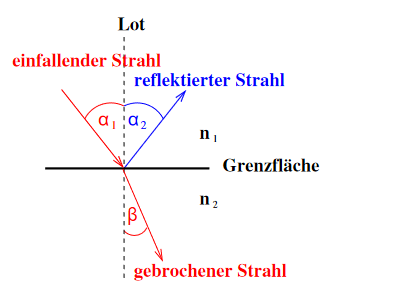
\includegraphics[width=5cm, keepaspectratio]{Reflexion und Brechung}
    \label{fig:Reflexion und Brechung}
    \caption{Reflexion und Brechung}
 \end{figure}
beschrieben. Für gewöhnlich wird Licht an Grenzflächen zwischen Materialien unterschiedlicher optischer Dichten teils reflektiert und teils transmittiert und gebrochen. Der Reflexionskoeffizient $R$ und der Transmissionskoeffizient $T$ sind definiert als das Verhältnis der reflektierten bzw. transmittierten Intensität zur einfallenden Intensität. Beide Koeffizienten müssen in Summe immer $1$ ergeben.
\subsection{Beugung}
Wenn Licht auf einen Spalt oder ein undurchlässiges Objekt trifft, breitet es sich im Schattenraum auf eine Weise aus, die durch die klassische Strahlenoptik nicht erklärbar ist.
Zur Erklärung dieser Beugung von Licht muss dieses als Welle mit einer bestimmten Frequenz bzw. Wellenlänge und Amplitude betrachtet werden. Wenn zwei Wellen überlagert werden addieren sich ihre Amplituden und es kommt zu Interferenz. Wenn die Wellen kohärent sind, also eine feste Phasenbeziehung besitzen und in ihrer Wellenlänge übereinstimmen führt dies je nach Gangunterschied zu einem bestimmten Interferenzbild. Dabei wird zwischen destruktiver und konstruktiver Interferenz unterschieden, wobei sich die Wellen bei ersterer gegenseitig abschwächen oder vollständig auslöschen, während sie sich bei zweiterer Verstärken. Wenn Licht auf einen Spalt trifft ist dieser gemäß des Huygensschen Prinzips Ausgangsort für eine Kugelfömige Elementarwelle. Bei einem optischen Gitter interferieren die einzelnen Elementarwellen und erzeugen ein Linienmuster als Interferenzbild. Dies ist dadurch zu erklären das nur für einige bestimmte Winkel ein Gangunterschied von $\Delta s=\lambda$ und somit konstruktive Interferenz zustande kommt, während bei den restlichen Winkeln destruktive Interferenz vorherscht. Die Lage des Maximums k-ter Ordnung wird durch
\begin{equation}
a\sin(\alpha)=k\lambda
\end{equation}
mit der Gitterkonstante $a$ beschrieben.
